\documentclass{article}
\usepackage[margin=1.0in]{geometry}
% \usepackage{amsmath, amsfonts, amssymb}
\usepackage[bookmarks=true, bookmarksopen=true, colorlinks=true]{hyperref}
\usepackage{graphicx}
\graphicspath{{./images}}
\usepackage{booktabs}
\usepackage{mathptmx}  % A Serif font
% \usepackage{helvet}  % A Sans-serif font. Requires switching to sans serif.
% \renewcommand{\familydefault}{\sfdefault}  % Switch to sans serif.
\usepackage[most]{tcolorbox}
\usepackage{algorithm}
\usepackage{algpseudocode}
\usepackage{caption}
\usepackage{subcaption}

\title{Geospatial Big Data Analysis - Lab 5}
\author{
    \textbf{Konstantinos Papadakis}\\
    National Technical University of Athens\\
    \texttt{k.i.papadakis@gmail.com}
}
\date{\vspace{-5ex}}

\begin{document}

\maketitle

\begin{abstract}
    In this document we train and evaluate a single-stage and a two-stage object detector on the \href{https://www.kaggle.com/datasets/markcsizmadia/object-detection-batteries-dices-and-toy-cars}{Batteries, Dice, and Toy Cars dataset}, and answer several questions regarding object detection deep learning models.
\end{abstract}

\section{The Dataset}
The dataset contains 640 by 640 resolution images which are annotated by axis-aligned rectangular regions containing a battery, dice, toy-car, candle, highlighter, or spoon. It is split into train, validation and test subsets, containing 1428, 102 and 123 images respectively. Samples from the dataset can be seen in Figure \ref{fig:one_of_each}. In Table \ref{table:counts}, the total number of objects for each class and in each subset is displayed.

\begin{table}[h]
    \centering
    \begin{tabular}{lrrrrrr}
        \toprule
                   & Battery & Dice & Toy-car & Candle & Highlighter & Spoon \\
        \midrule
        Train      & 830     & 768  & 647     & 101    & 90          & 46    \\
        Validation & 42      & 65   & 59      & 0      & 0           & 0     \\
        Test       & 52      & 62   & 49      & 0      & 0           & 0     \\
        Total      & 924     & 895  & 755     & 101    & 90          & 46    \\
        \bottomrule
    \end{tabular}
    \caption{Class representation across the images of the dataset}
    \label{table:counts}
\end{table}

\begin{figure}[h]
    \centering
    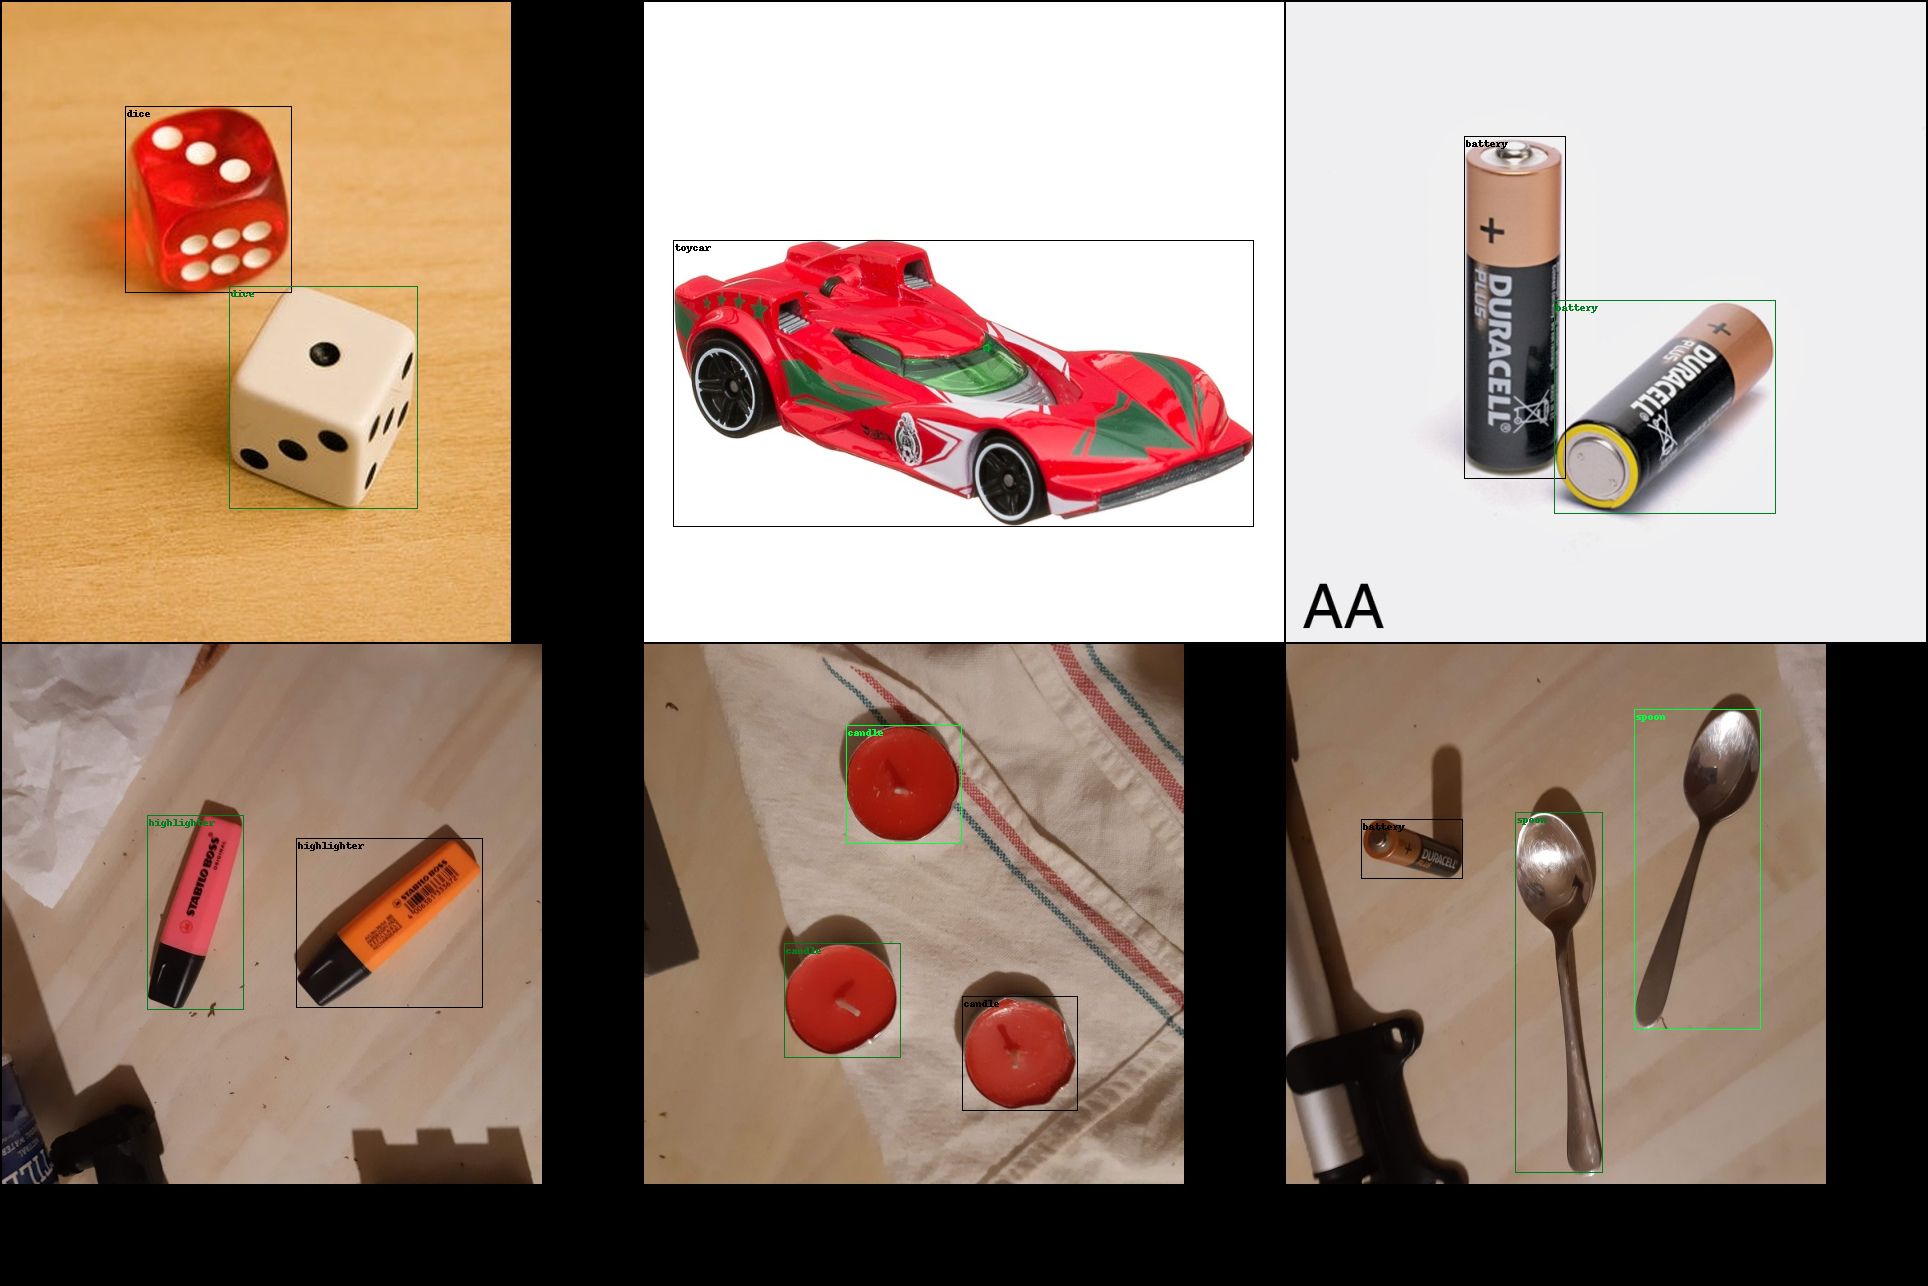
\includegraphics[width=\textwidth]{one_of_each.png}
    \caption{Images from the training set, with box annotations. All classes represented.}
    \label{fig:one_of_each}
\end{figure}

\section{Object Detection}

We train, evaluate and compare a two stage detector in the form of Faster R-CNN and a single stage detector in the form of RetinaNet. Both models use a ResNet50 pre-trained on ImageNet to create their feature pyramid network (FPN). Also, in both models, the trainable layers of the ResNet50 are the final 3 out of the 5 total.

During training, we load images in batches of size 8, and augment them by sequentially applying each one of the following transforms with probability 0.5:
\begin{itemize}
    \item A horizontal flip.
    \item A random rotation by a right angle, zero or more times.
    \item A random change in brightness and in contrast by a factor in \([-0.2, 0.2]\).
\end{itemize}

\subsection{One-Stage Detector (RetinaNet)}
We train a RetinaNet \cite{retinanet} with a setting of 110 epochs maximum and early stopping. More specifically, during training, every half epoch we evaluate the mean average precision (mAP) on the validation set. If the mAP didn’t improve for 30 consecutive half-epochs, we stop the training early. Early stopping did happen on epoch 103, meaning that the best weights were achieved on epoch 89. A learning rate of 0.0001 was used.

\subsection{Two-Stage Detector (Faster R-CNN)}

We train a Faster R-CNN using the 4-Step Alternating Training described in the original paper \cite{fasterrcnn}.

\begin{enumerate}
    \item In step-1 we initialize and train a model that is composed of just the backbone and the region proposal network (RPN). When step-1 is finished, we call the model to create and cache proposals which we will use in step-2.
    \item In step-2 we initialize a model composed of a \emph{new} backbone and the Region of Interest (ROI) Heads. The proposals that we use are the ones cached from step-1.
    \item In step-3 the model is composed of the step-2 backbone and the step-1 RPN. We update only the RPN weights and keep the backbone frozen.
    \item In step-4 the model is composed of all the Faster R-CNN parts (Backbone, RPN, ROI Heads). We update only the ROI Heads weights and keep the backbone and the RPN frozen.
\end{enumerate}

Steps 1, 2 and 3 were trained for 20 epochs. Step-4 was trained with a setting of 50 epochs maximum, and with the same early stopping strategy that was used for RetinaNet. Early stopping did happen on epoch 32, meaning that the best weights were achieved on epoch 17. In all steps, a learning rate of 0.0001 was used.

\section{Results}
For a summary of the results, see Table \ref{table:test_map}. We observe that the models performed equally well overall. One noticable difference is that RetinaNet seems to perform significantly better on medium sized objects, compared to Faster R-CNN (0.931 mAP vs 0.899 mAP).

More detailed results can be found in the images of Appendix \ref{appendix:results}. To interactively explore the learning curves of the appendix, one can visit \href{https://tensorboard.dev/experiment/ErXpnafeS6aX9Fleh9lCZQ/}{tensorboard.dev}. To be able to interactively explore the predicted images as well, it is possible to download the \href{https://ntuagr-my.sharepoint.com/:u:/g/personal/konstantinospapadakis_ntua_gr/EdNjt6ZTrDlPtkvl6aJubhsB8nTLo-kJOdELaH411BjGmg?e=64G3z5}{tensorboard logs} and instantiate a local tensorboard server.

\begin{table}[h]
    \centering
    \begin{tabular}{lrr}
        \toprule
                        & Faster R-CNN & RetinaNet \\
        Metric          &              &           \\
        \midrule
        mAP             & 0.892        & 0.897     \\
        mAP@50          & 0.998        & 0.983     \\
        mAP@75          & 0.973        & 0.983     \\
        mAP battery     & 0.861        & 0.873     \\
        mAP dice        & 0.914        & 0.929     \\
        mAP toycar      & 0.900        & 0.890     \\
        mAP large       & 0.905        & 0.903     \\
        mAP medium      & 0.877        & 0.915     \\
        mAP small       & -1.000       & -1.000    \\
        mAR@1           & 0.672        & 0.675     \\
        mAR@10          & 0.913        & 0.922     \\
        mAR@100         & 0.913        & 0.922     \\
        mAR@100 battery & 0.887        & 0.904     \\
        mAR@100 dice    & 0.932        & 0.945     \\
        mAR@100 toycar  & 0.920        & 0.918     \\
        mAR large       & 0.922        & 0.924     \\
        mAR medium      & 0.899        & 0.931     \\
        mAR small       & -1.000       & -1.000    \\
        \bottomrule
    \end{tabular}
    \caption{Evaluation results on the test set. For the mean average recall see \cite{mar}.}
    \label{table:test_map}
\end{table}

\section{Questions}

\subsection{Question 1}
\begin{tcolorbox}
    Is the mean average precision a good metric for early stopping during RPN training?
\end{tcolorbox}
It is indeed. We calculate the mAP as per usual with the number of classes being equal to 1 (the “object” class) and on multiple intersection over union (IoU) thresholds, e.g. \(\{0.5, 0.55, \dots, 0.95\}\). More explicitly, we follow the steps in Algorithm \ref{algorithm:mAP}.
\begin{algorithm}[h]
    \begin{algorithmic}[1]
        \For{each threshold in IoU thresholds}
        \State{Sort the proposals descendingly by their objectness score.}
        \State{Initialize a set containing the ground truths.}
        \State{Initialize a precision-recall curve.}
        \For{each proposed box}
        \If{the proposed box has IoU greater than the threshold with at least one ground truth box}
        \State{Consider the proposal as a true positive.}
        \State{Delete the ground truth box with the highest IoU from the current set of ground truths.}
        \Else
        \State{Consider the proposal as a false positive.}
        \EndIf
        \State{Calculate the current precision and recall, and plot a point on the precision-recall curve.}
        \EndFor
        \State{Calculate the average precision, that is the area under the precision-recall curve.}
        \EndFor
        \State{Calculate the mAP, which is the mean of the average precisions over all IoU thresholds.}
    \end{algorithmic}
    \caption{mAP computation for the RPN}
    \label{algorithm:mAP}
\end{algorithm}

\subsection{Question 2}
\begin{tcolorbox}
    Say an object detection model predicts the classes with high accuracy but the proposed boxes have relatively low IoU with the ground truth ones. How could this issue be ameliorated?
\end{tcolorbox}
We can give more importance to the box regression loss by changing the loss function
from \(\text{Loss}_\text{box regressor}\ +\ \text{Loss}_\text{classifier}\)
to \(a\ \text{Loss}_\text{box regressor}\ +\ \text{Loss}_\text{classifier}\)
where \(a > 1\).

\subsection{Question 3}
\begin{tcolorbox}
    Say we have images of a 100m part of a highway, with the images being taken from a UAV in 2840 by 2160 (4K) resolution. What issues would be encountered in attempting to detect cars with a model like Faster R-CNN or RetinaNet?
\end{tcolorbox}
Typical object detector architectures use backbones that work with small or medium sized images. If we feed a 4K image to a Resnet50 we would end up with a large number of features which would mean a very large number of proposals, which would be hard to handle. A naive approach to solving this issue is to resize the image down to a lower resolution, but this would mean that information about small objects would be lost and it would make it harder or even impossible to detect them. Another approach would be to use an algorithm like Slicing-Aided Hyper Inference (SAHI) \cite{sahi} where we perform the detection on crops of the original image and then combine the results.

\subsection{Question 4}
\begin{tcolorbox}
    Say we want to use a model like Faster R-CNN or RetinaNet to perform detection of all people in a dense concert crowd. What issue would be encountered?
\end{tcolorbox}
The model would probably not perform very well due to the nature of greedy algorithms like Non Max Suppression (NMS) which are typically used to prune “duplicate” proposals from the RPN (and detections from the ROI Heads). The NMS algorithm would repeatedly find the proposal with the highest objectness score and remove all other proposals with IoU higher than some predefined threshold. The issue arises from the fact that in a crowd, the IoU between ground truth boxes is high, which means that the NMS algorithm would suppress “good” proposals. Setting the IoU threshold high would result in many “duplicate” proposals, while setting the IoU threshold low would result in removing many “good” proposals.



\bibliographystyle{IEEEtran}
\bibliography{refs}

\appendix

\section{Detailed Results}
\label{appendix:results}

\begin{figure}[h]
    \centering
    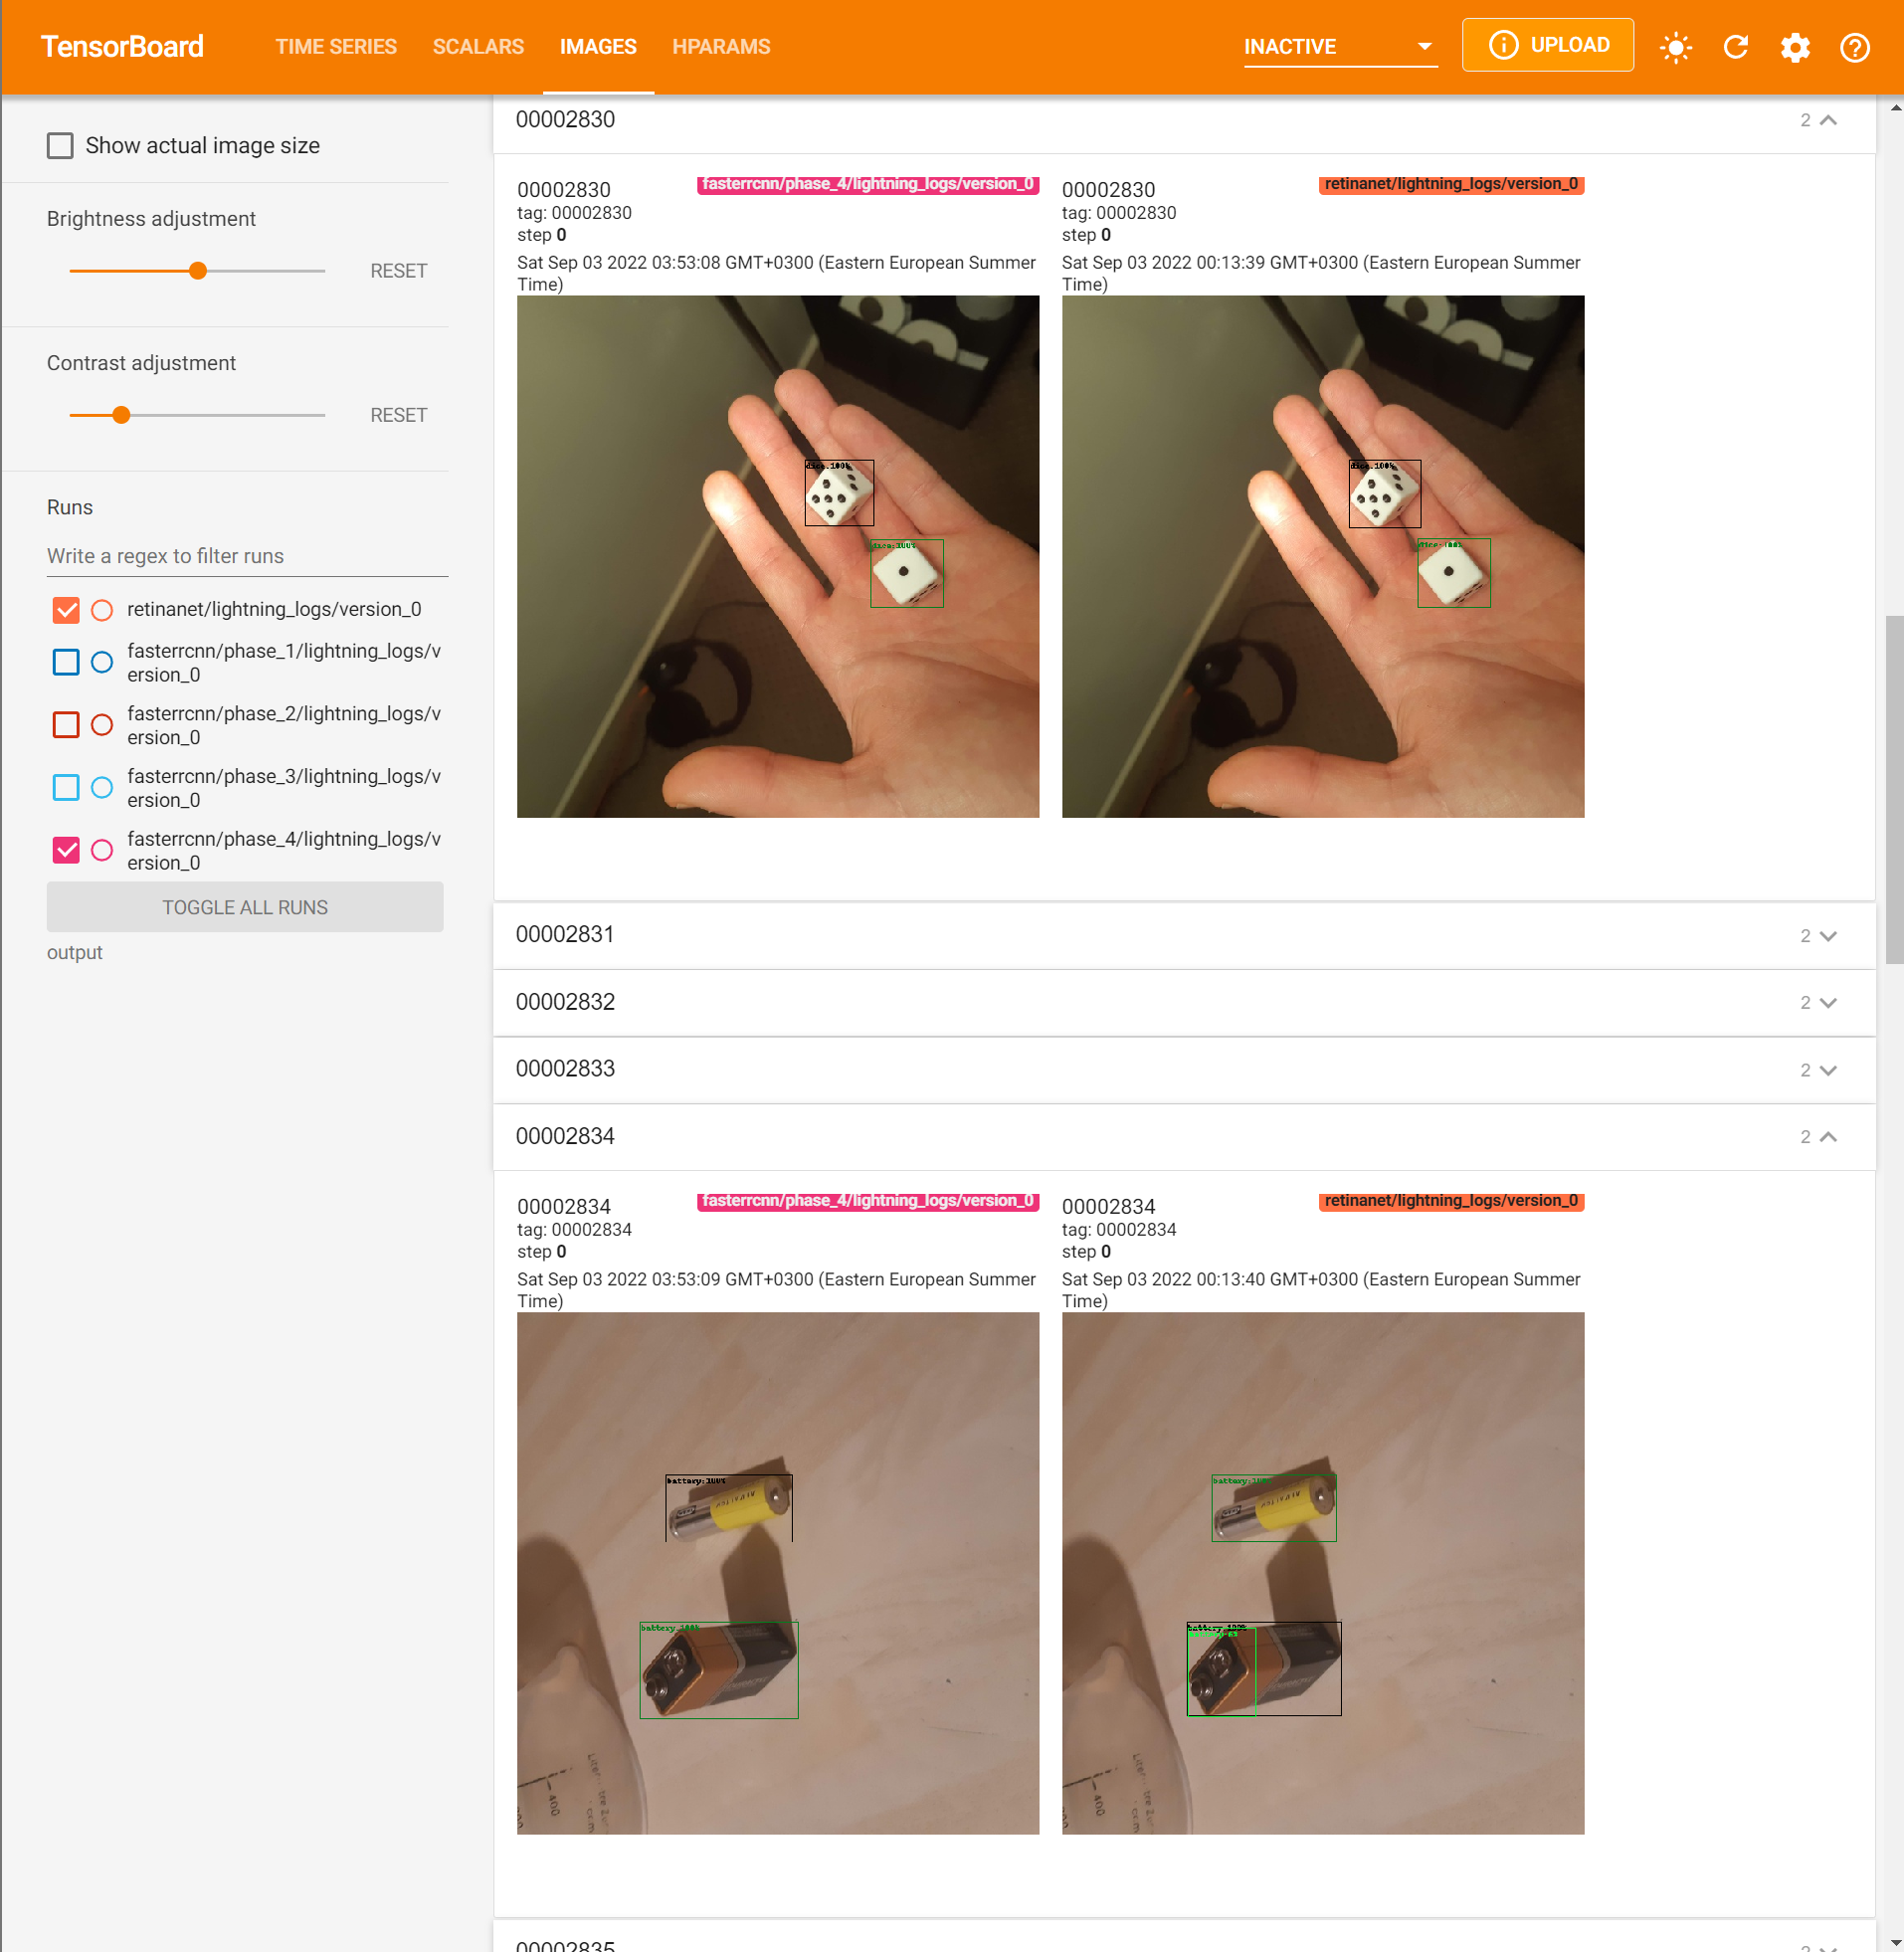
\includegraphics[width=\textwidth]{tensorboard_screenshots/predictions.png}
    \caption{Predictions of Faster R-CNN phase 4, and RetinaNet.}
    \label{fig:predictions}
\end{figure}

\begin{figure}[h]
    \centering
    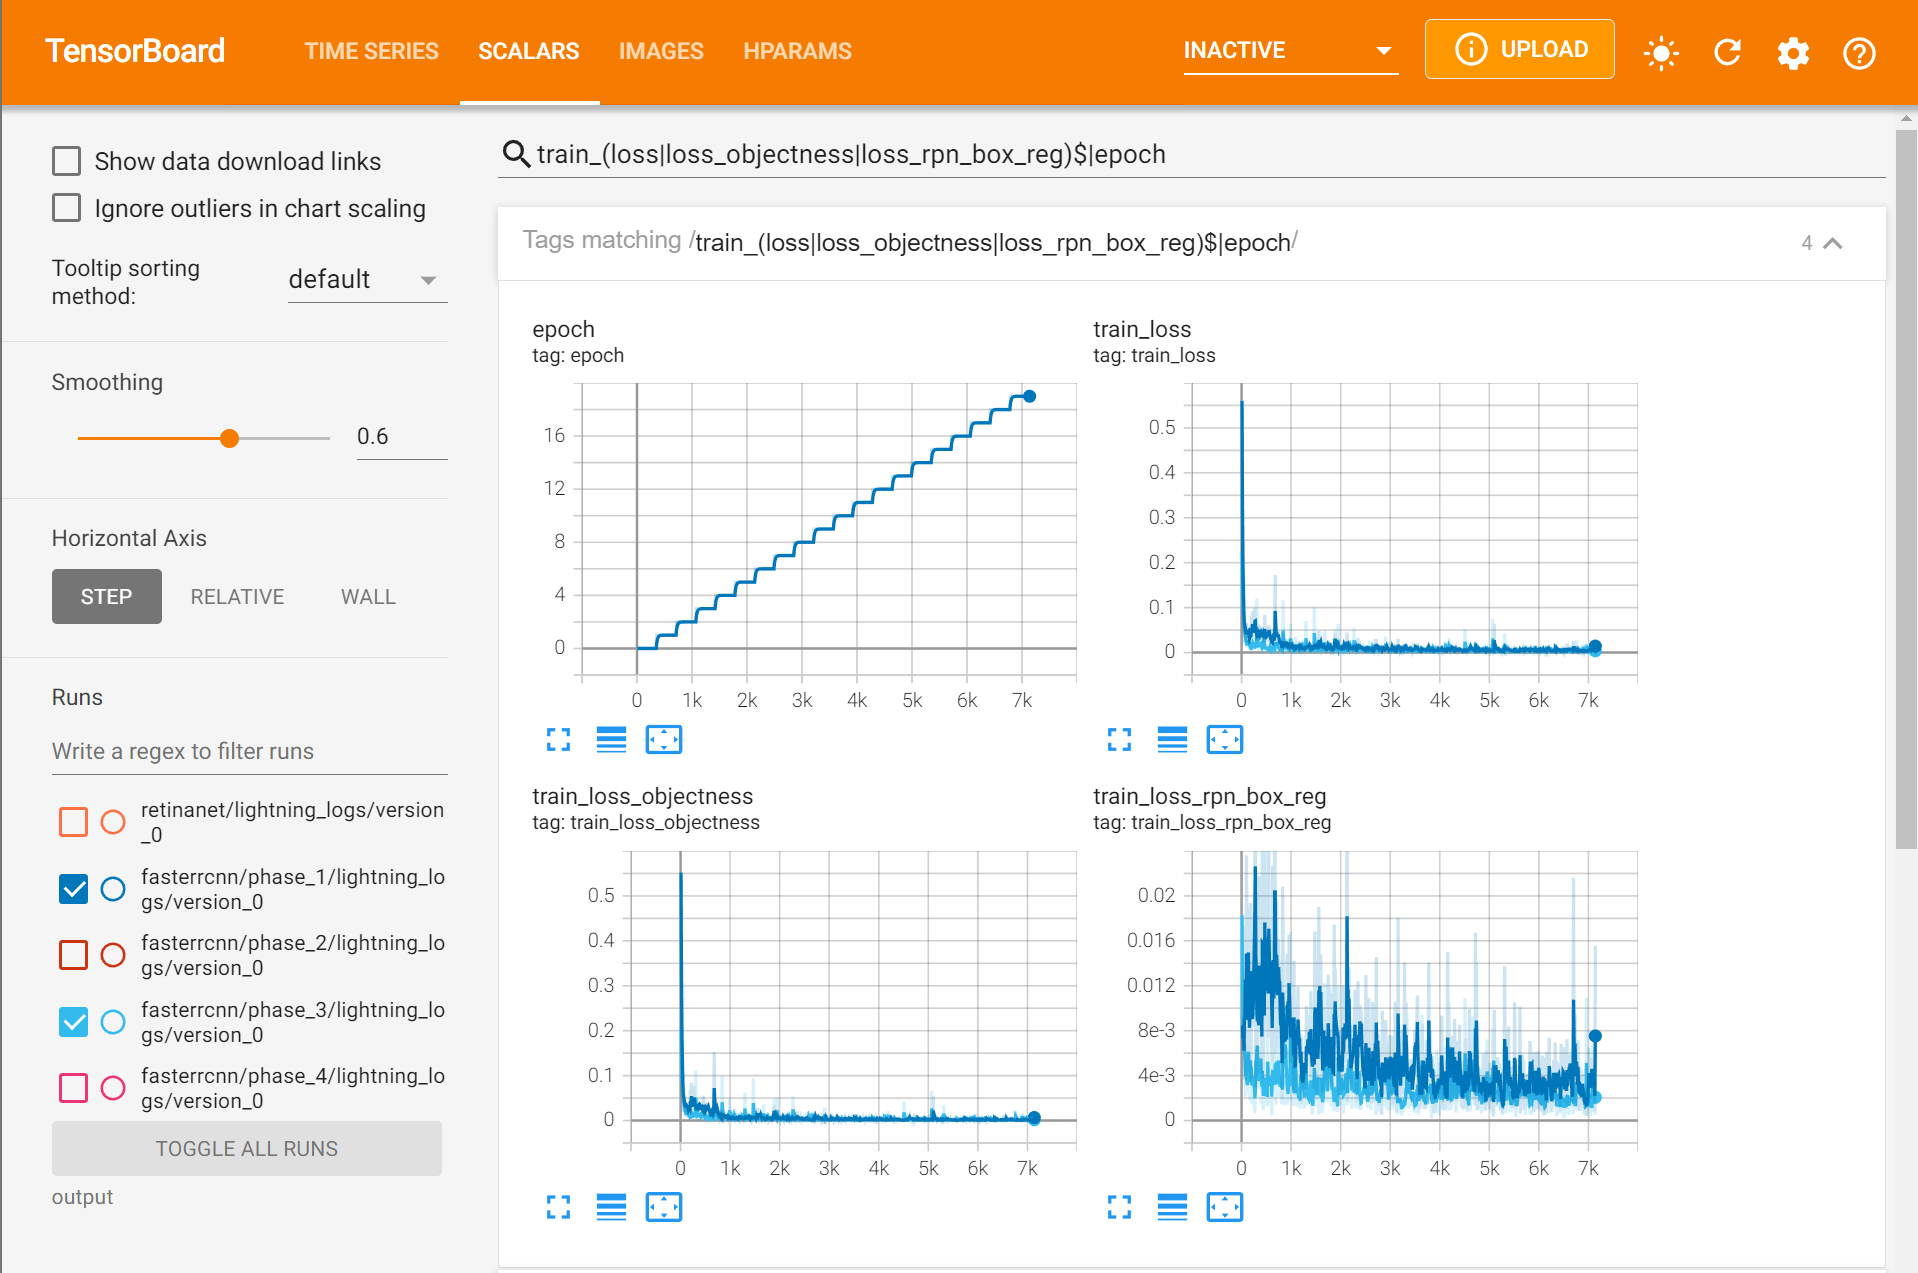
\includegraphics[width=\textwidth]{tensorboard_screenshots/train_losses_p13.png}
    \caption{Training loss curves of Faster R-CNN phases 1 and 3.}
    \label{fig:train_losses_p13}
\end{figure}

\begin{figure}[h]
    \centering
    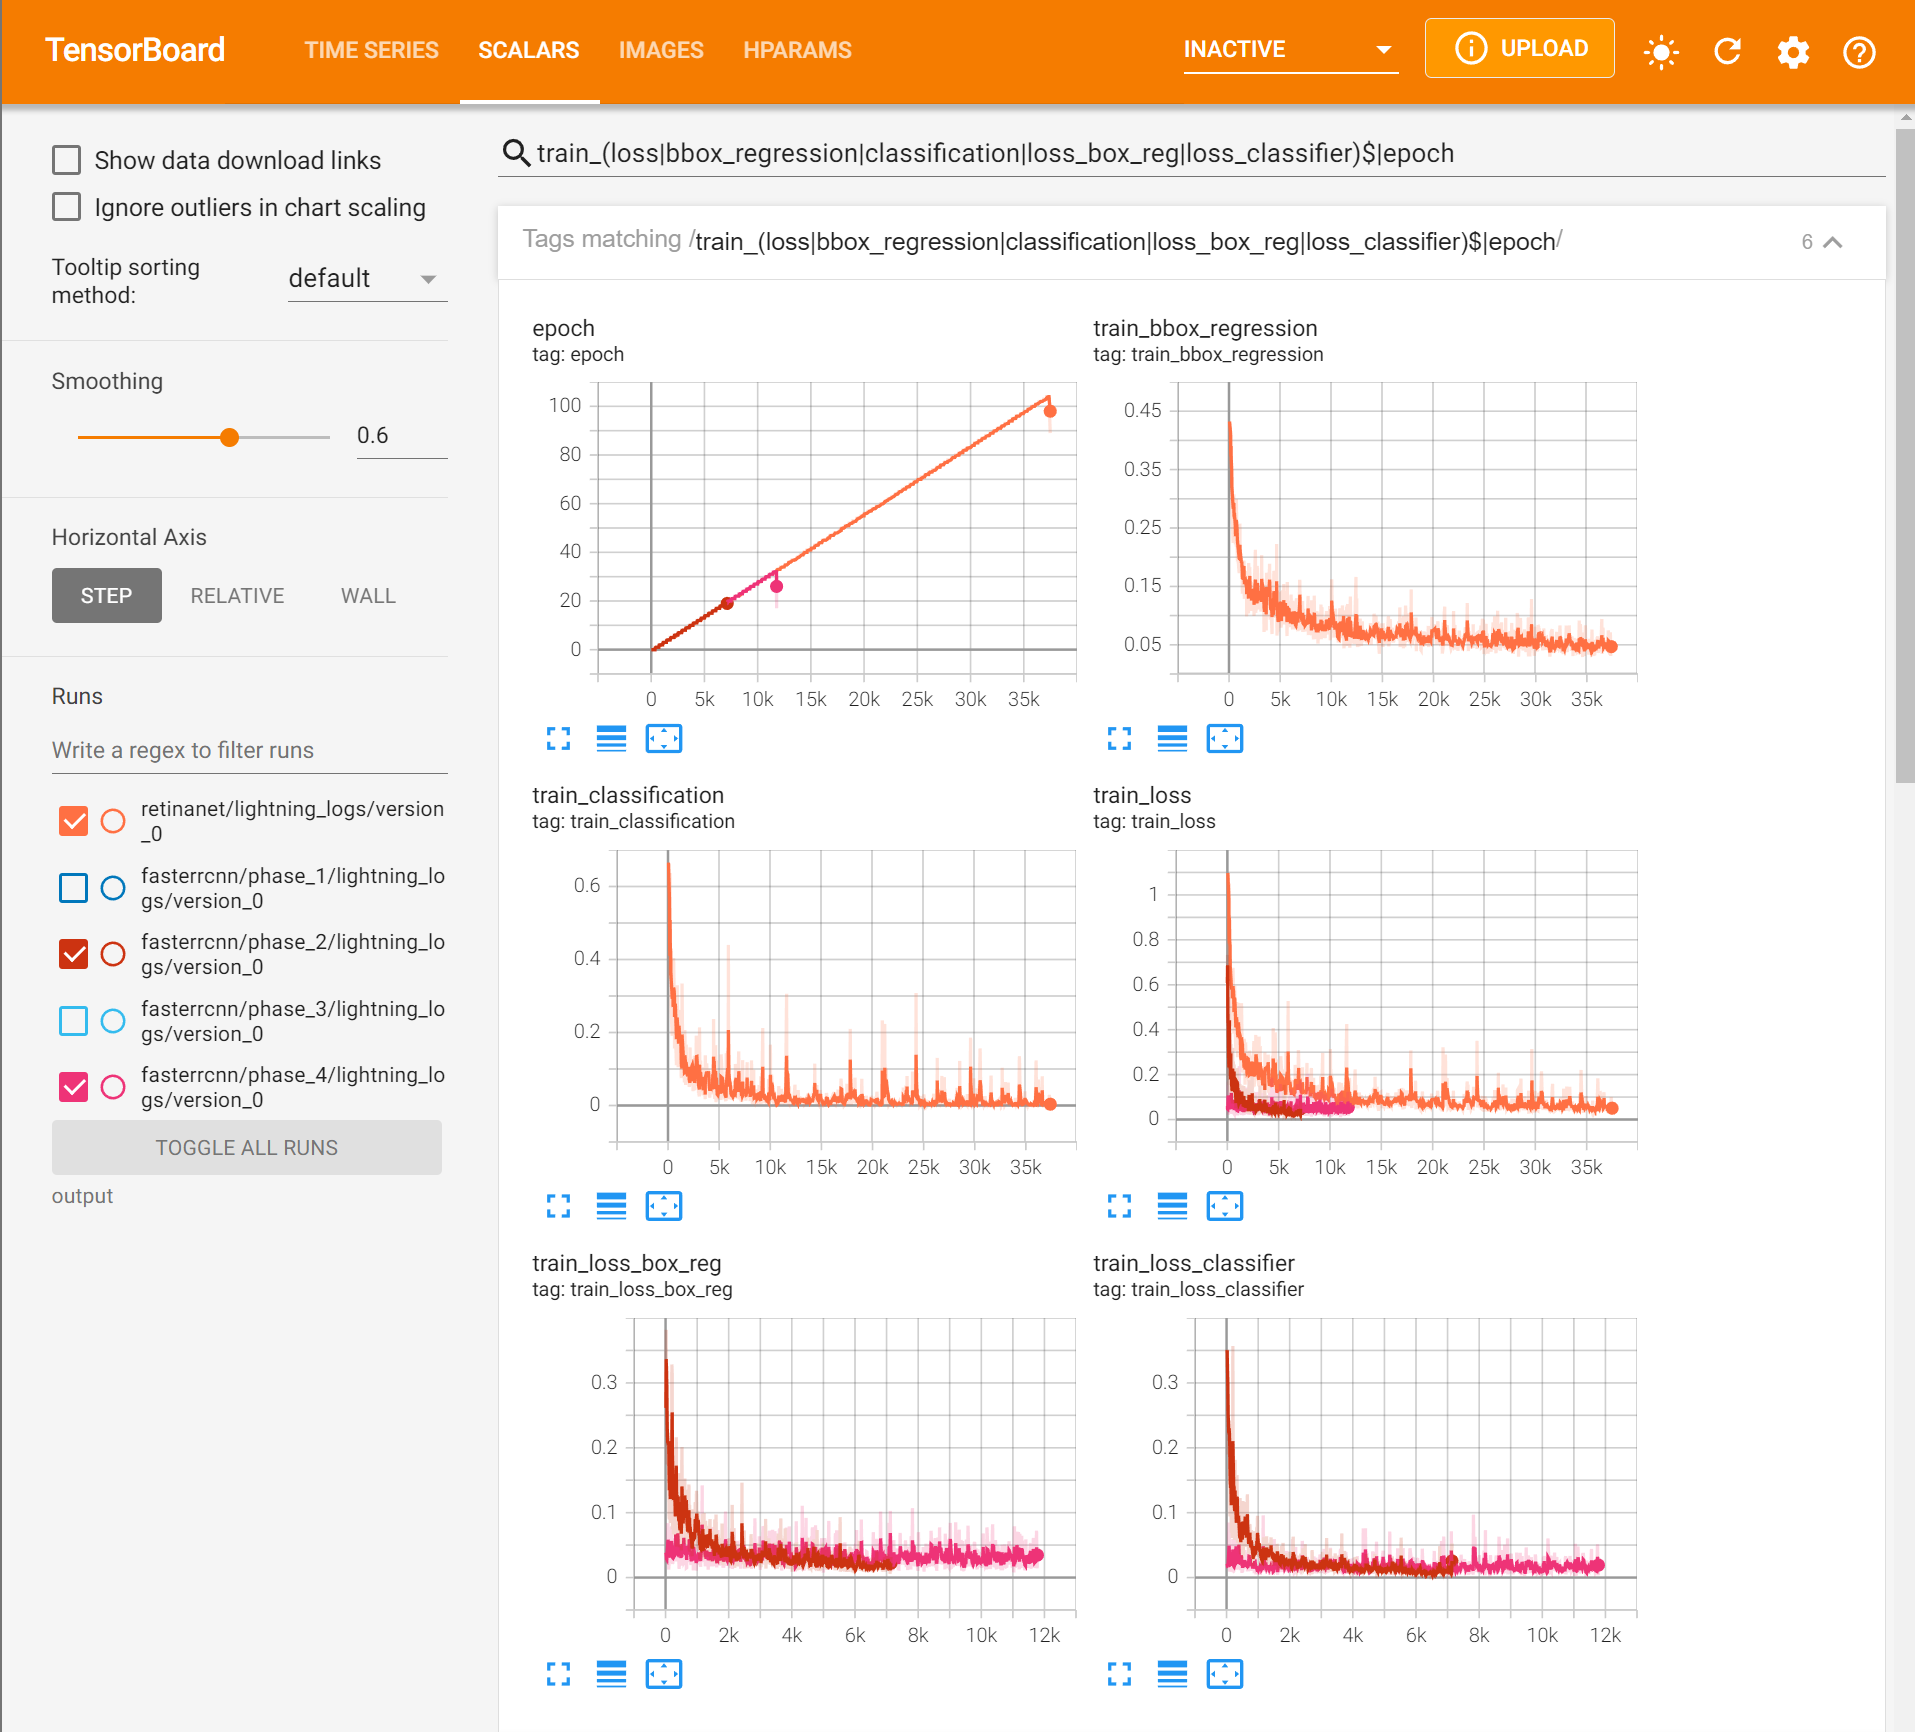
\includegraphics[width=\textwidth]{tensorboard_screenshots/train_losses_p24r.png}
    \caption{Training loss curves of Faster R-CNN phases 2 and 4, and RetinaNet}
    \label{fig:train_losses_p24r}
\end{figure}

\begin{figure}[h]
    \centering
    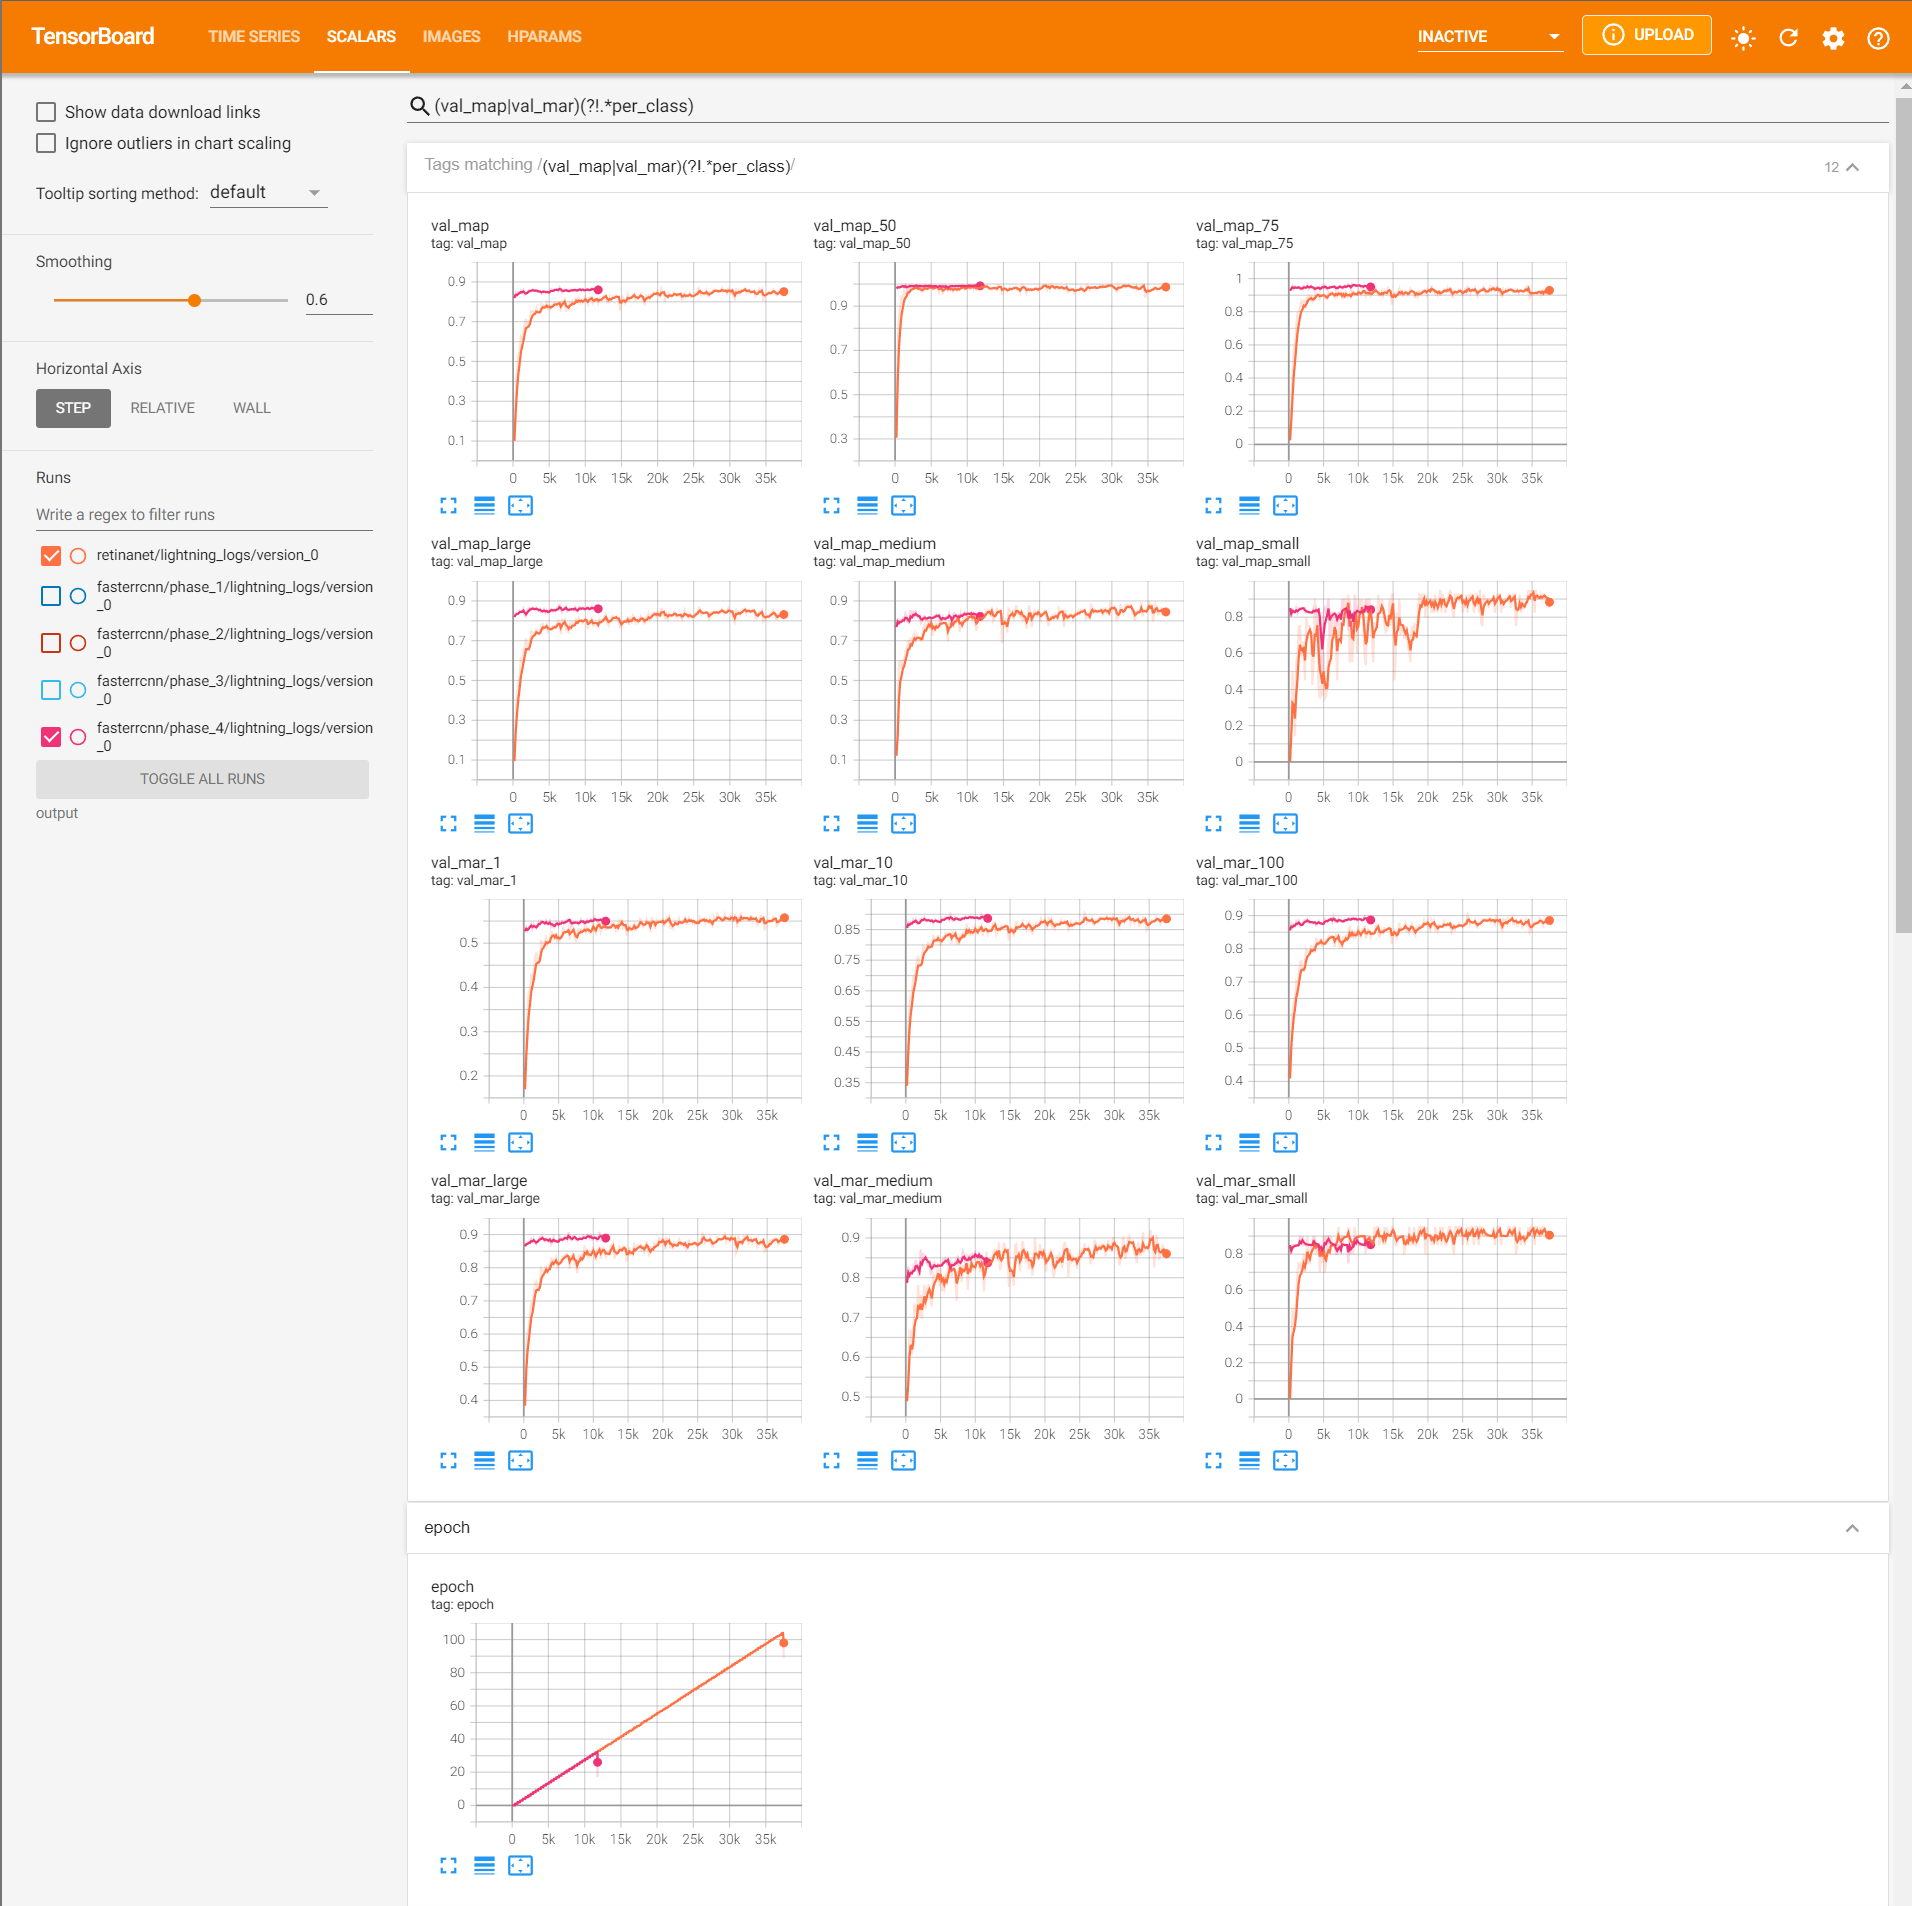
\includegraphics[width=\textwidth]{tensorboard_screenshots/val_map.png}
    \caption{Validation mAP curves of Faster R-CNN phase 4 and RetinaNet}
    \label{fig:val_map}
\end{figure}

\begin{figure}[h]
    \centering
    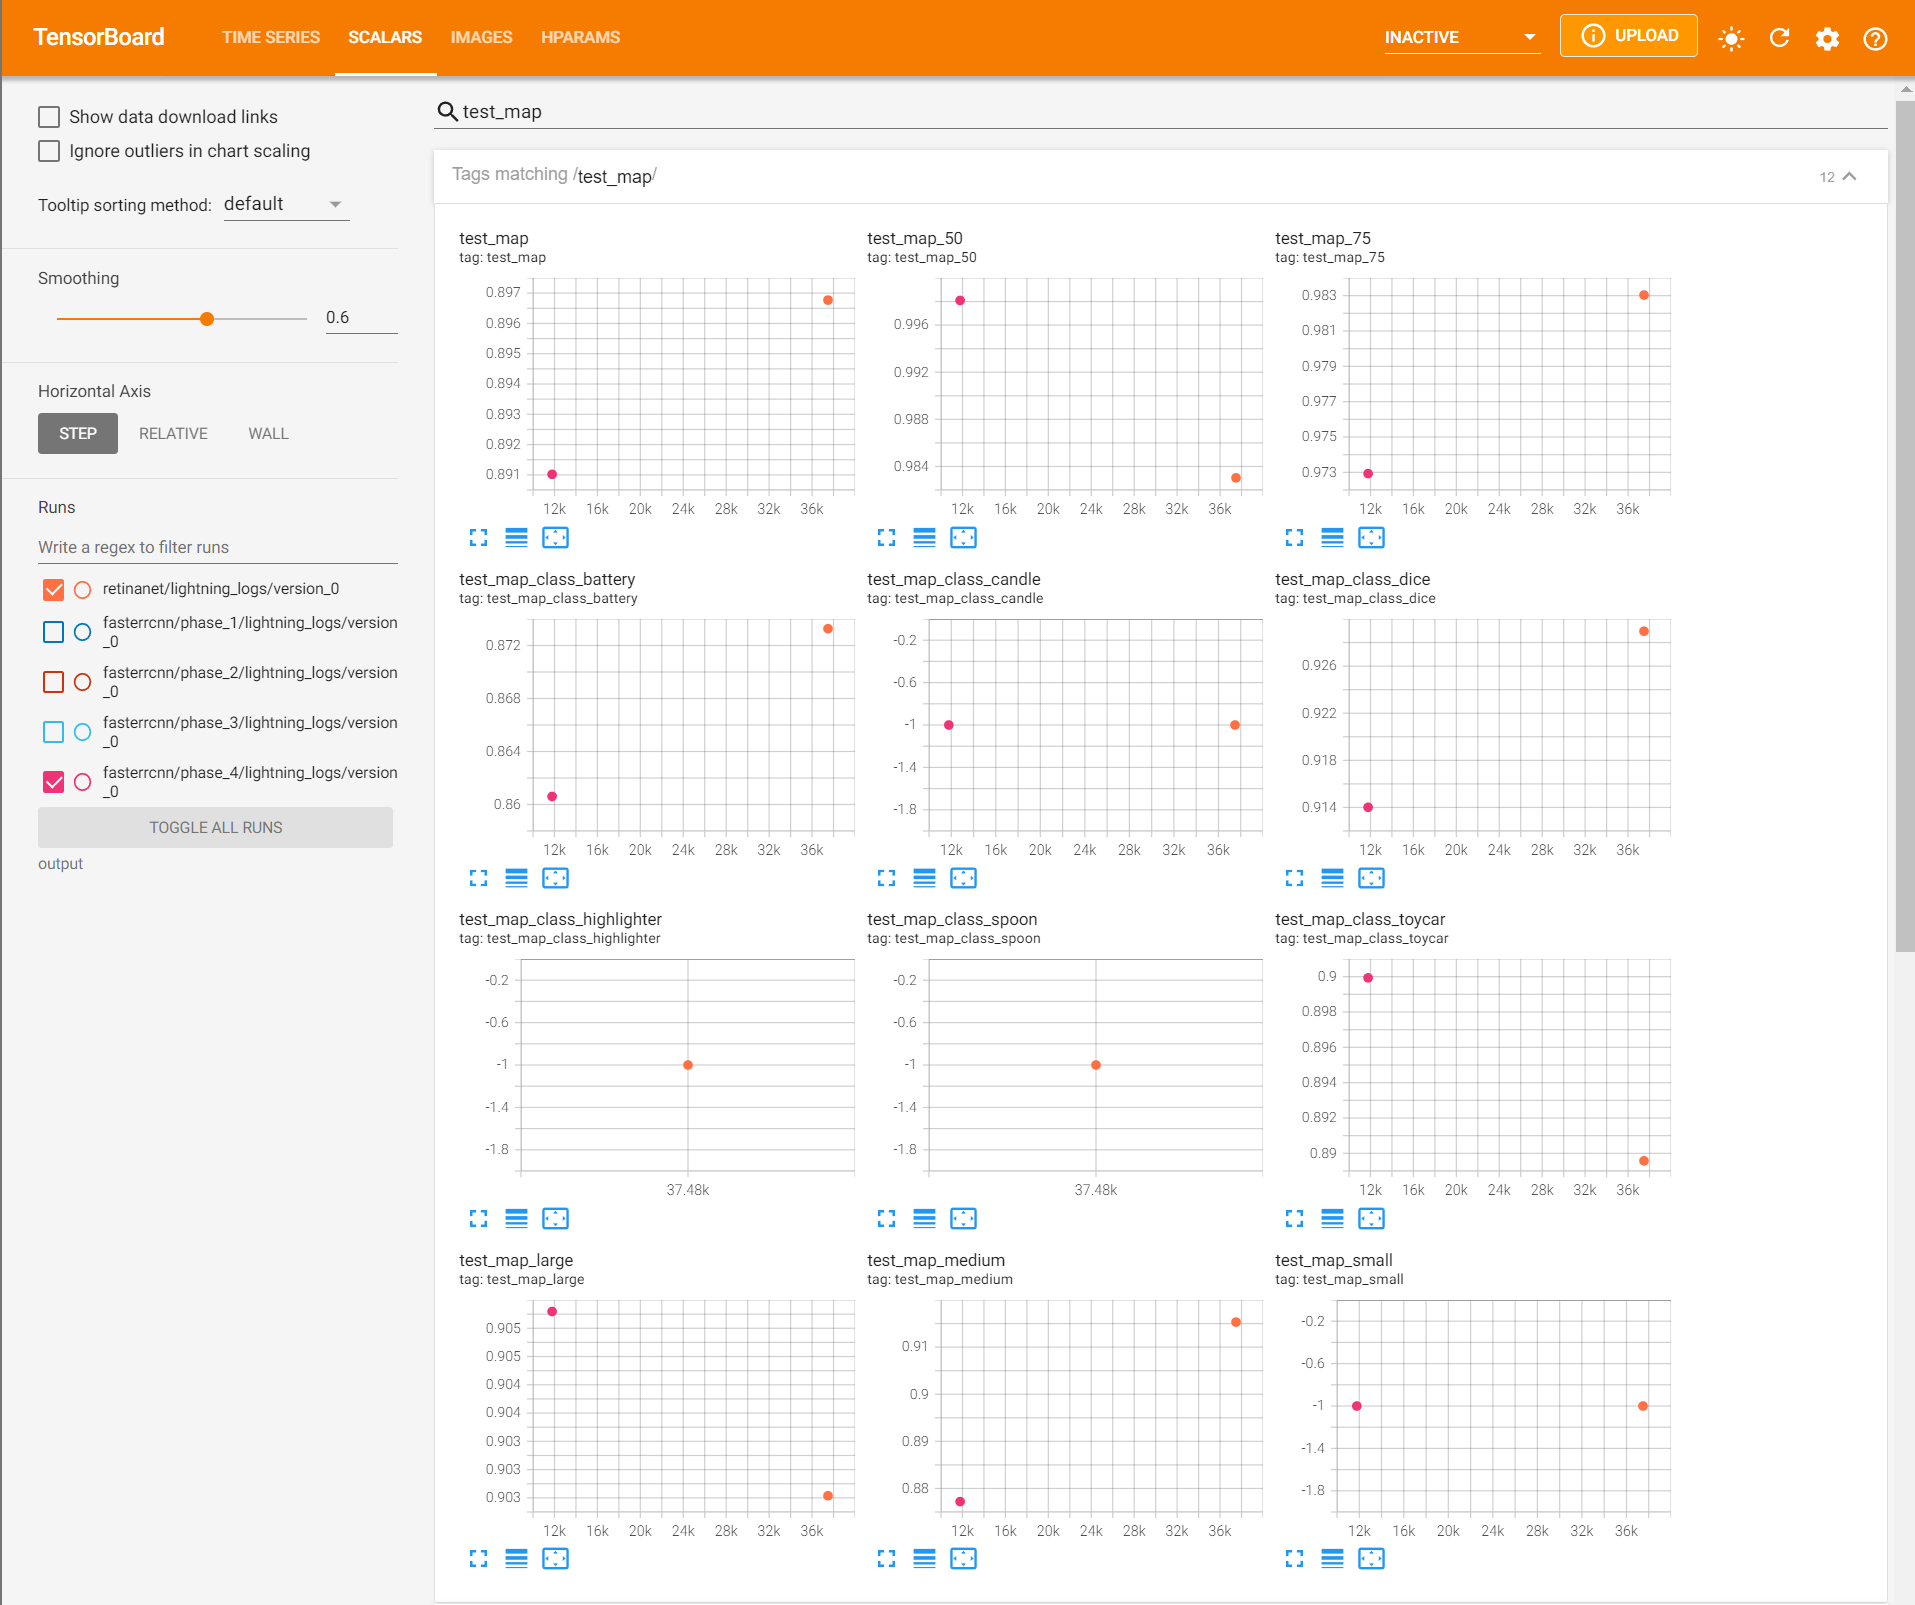
\includegraphics[width=\textwidth]{tensorboard_screenshots/test_map.png}
    \caption{Test mAP of Faster R-CNN phase 4 and RetinaNet}
    \label{fig:test_map}
\end{figure}

\newcommand{\plotpreds}[1]{
    \begin{figure}
        \centering

        \begin{subfigure}[b]{0.49\textwidth}
            \centering
            \includegraphics[width=\textwidth]{#1_fasterrcnn.png}
            \caption{Faster R-CNN}
            \label{fig:#1_fasterrcnn}
        \end{subfigure}
        \hfill
        \begin{subfigure}[b]{0.49\textwidth}
            \centering
            \includegraphics[width=\textwidth]{#1_retinanet.png}
            \caption{RetinaNet}
            \label{#1_retinanet}
        \end{subfigure}

        \caption{#1.png}
        \label{fig:#1}
    \end{figure}
}

\plotpreds{00002806}
\plotpreds{00002812}
\plotpreds{00002843}
\plotpreds{00002852}
\plotpreds{00002863}
\plotpreds{00002884}
\plotpreds{00002894}
\plotpreds{00002898}

\end{document}
